%% Creator: Inkscape inkscape 0.48pre0, www.inkscape.org
%% PDF/EPS/PS + LaTeX output extension by Johan Engelen, 2010
%% Accompanies image file 'h_separation' (pdf, eps, ps)
%%
%% To include the image in your LaTeX document, write
%%   \input{<filename>.tex}
%%  instead of
%%   \includegraphics{<filename>.pdf}
%% To scale the image, write
%%   \def{\svgwidth}{<desired width>}
%%   \input{<filename>.tex}
%%  instead of
%%   \includegraphics[width=<desired width>]{<filename>.pdf}

\begingroup
  \makeatletter
  \providecommand\color[2][]{%
    \errmessage{(Inkscape) Color is used for the text in Inkscape, but the package 'color.sty' is not loaded}
    \renewcommand\color[2][]{}%
  }
  \providecommand\transparent[1]{%
    \errmessage{(Inkscape) Transparency is used (non-zero) for the text in Inkscape, but the package 'transparent.sty' is not loaded}
    \renewcommand\transparent[1]{}%
  }
  \providecommand\rotatebox[2]{#2}
  \ifx\svgwidth\undefined
    \setlength{\unitlength}{335pt}
  \else
    \setlength{\unitlength}{\svgwidth}
  \fi
  %\setlength{\baseline}{0.04}
  \global\let\svgwidth\undefined
  \makeatother
  \begin{picture}(1,1.61179619)%
    \put(0,0){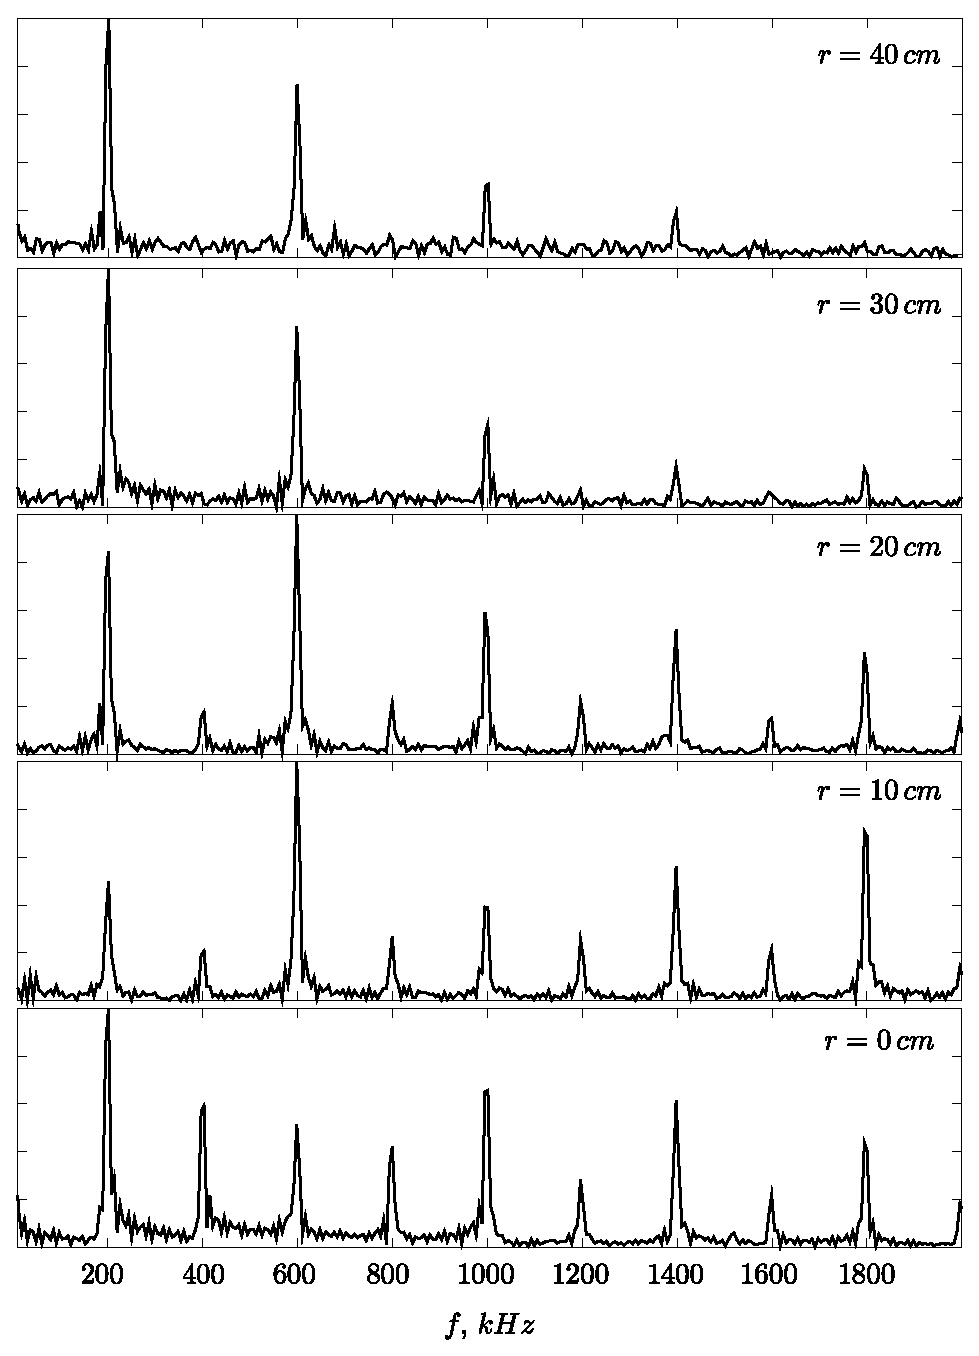
\includegraphics[width=\unitlength]{pics/h_separation.eps}}%
    \put(0.07,-0.04459907){\makebox(0,0)[lb]{\smash{$200$}}}%
    \put(0.168,-0.04459907){\makebox(0,0)[lb]{\smash{$400$}}}%
    \put(0.266,-0.04459907){\makebox(0,0)[lb]{\smash{$600$}}}%
    \put(0.368,-0.04459907){\makebox(0,0)[lb]{\smash{$800$}}}%
    \put(0.458,-0.04459907){\makebox(0,0)[lb]{\smash{$1000$}}}%
    \put(0.556,-0.04459907){\makebox(0,0)[lb]{\smash{$1200$}}}%
    \put(0.654,-0.04459907){\makebox(0,0)[lb]{\smash{$1400$}}}%
    \put(0.756,-0.04459907){\makebox(0,0)[lb]{\smash{$1600$}}}%
    \put(0.854,-0.04459907){\makebox(0,0)[lb]{\smash{$1800$}}}%
    \put(0.436,-0.12){\makebox(0,0)[lb]{\smash{$f$\,(кГц)}}}%
    \put(-0.1,-0.005 ){\makebox(0,0)[lb]{\smash{$-40$}}}%
    \put(-0.1,0.07){\makebox(0,0)[lb]{\smash{$-30$}}}%
    \put(-0.1,0.15){\makebox(0,0)[lb]{\smash{$-20$}}}%
    \put(-0.1,0.227){\makebox(0,0)[lb]{\smash{$-10$}}}%
    \put(-0.05,0.3){\makebox(0,0)[lb]{\smash{$0$}}}%
    \put(-0.15,0.78){\rotatebox{90}{\makebox(0,0)[lb]{\smash{$A$\,(дБ)}}}}%

    \put(0.8,0.27){\makebox(0,0)[lb]{\smash{$r=0$\,cм}}}%

    \put(-0.1,0.41){\makebox(0,0)[lb]{\smash{$-30$}}}%
    \put(-0.1,0.488){\makebox(0,0)[lb]{\smash{$-20$}}}%
    \put(-0.1,0.565){\makebox(0,0)[lb]{\smash{$-10$}}}%
    \put(-0.05,0.638){\makebox(0,0)[lb]{\smash{$0$}}}%

    \put(0.8,0.60){\makebox(0,0)[lb]{\smash{$r=10$\,см}}}%
    \put(-0.1,0.745){\makebox(0,0)[lb]{\smash{$-30$}}}%
    \put(-0.1,0.825){\makebox(0,0)[lb]{\smash{$-20$}}}%
    \put(-0.1,0.905){\makebox(0,0)[lb]{\smash{$-10$}}}%
    \put(-0.05,0.975){\makebox(0,0)[lb]{\smash{$0$}}}%
   
    \put(0.8,0.94){\makebox(0,0)[lb]{\smash{$r=20$\,см}}}%
    \put(-0.1,1.085){\makebox(0,0)[lb]{\smash{$-30$}}}%
    \put(-0.1,1.165){\makebox(0,0)[lb]{\smash{$-20$}}}%
    \put(-0.1,1.242){\makebox(0,0)[lb]{\smash{$-10$}}}%
    \put(-0.05,1.315){\makebox(0,0)[lb]{\smash{$0$}}}%
   
    \put(0.8,1.28){\makebox(0,0)[lb]{\smash{$r=30$\,см}}}%
    \put(-0.1,1.42){\makebox(0,0)[lb]{\smash{$-30$}}}%
    \put(-0.1,1.5){\makebox(0,0)[lb]{\smash{$-20$}}}%
    \put(-0.1,1.584){\makebox(0,0)[lb]{\smash{$-10$}}}%
    \put(-0.05,1.655){\makebox(0,0)[lb]{\smash{$0$}}}%
   
    \put(0.8,1.615){\makebox(0,0)[lb]{\smash{$r=40$\,см}}}%
  \end{picture}%
\endgroup
